\chapter{Реализация норадреналиновой системы}
\label{chap:specification}
Норадреналиновая система являлась последним недостающим элементом когнитивной архитектуры NeuCogAr, при уже реализованных дофаминовой и серотониновой системах. В этой главе описываются базовые принципы динамики концентрации норадреналина, их программная реализация и тестирование.

Нейромодулятор норадреналин (он же норэпинефрин) относится к биогенным аминам, группе катехоламинов, он активно используется симпатической периферийной нервной системой (мобилизует организм к действию) и центральной нервной системой (мобилизует мозг для действий).\cite{noradrenalin3} Норадренергические нейроны в мозге немногочисленны: около 4000 в основном месте залегания — голубоватом пятне (locus coeruleus), около 3000 в ядрах солитарного тракта (nucleus tractus solitarii).\cite{masuko, rat_data5} Но эти нейроны посылают проекции во многие области мозга и оказывают на них значительное влияние. Активность норадренергических нейронов связана с разнообразными реакциями: на стресс, на неожиданность, на такие раздражители как боль, жар или холод, затруднение дыхания. Во время сна активность в очаге голубоватого пятна падает, во время бодрствования работает на уровне минимально необходимом, резко повышается при появлении стимула, привлекающего внимание.\cite{Berridge2003} Высокий уровень норадреналина вызывает повышение бдительности и скорости реакции, фокусировку внимания, улучшение обработки сенсорных входов, повышение уровня возбуждения.


Контроль над такими когнитивными процессами как внимание, возбуждение и бдительность необходим для реализации эмоциональных состояний злости, удивления, страдания и заинтересованности. Поэтому, по аналогии с существующими моделями дофамина и серотонина, принципы работы норадреналина были реализованы в виде нового модуля, добавленного в NEST Simulator.


Модель механизма изменения концентрации норадреналина основана на модели, предложенной Е. Ижикевичем для описания динамики концентрации дофамина после серии событий (поощрений).\cite{izhikevich} В работе Е. Ижикевича принципы всплеска дофамина в ответ на поощрение иллюстрируются собаками Павлова, вырабатывавшими рефлексы в связи с тем, какие действия сопровождались наградой. Исследуя механизм вырабатываемого рефлекса, неясно, как мозг «запоминает» цепочки нейронов, активность которых вознаграждалась - ведь между событием и наградой проходило несколько секунд (слишком долго для стандартного алгоритма спайковой пластичности).


Е. Ижикевич вводит понятие «сигнализирующей отметки» (eligibility trace) — своеобразных следов, оставляемых в синапсе после того, как по нему проходит спайк. В реальном биологическом мозге это какие-либо кислоты, активизируемые ненадолго, но дольше, чем на пару секунд. Затем, как проиллюстрировано на \ref{fig:izhikevich}, награда (поощрение) вызывает резкое повышение уровня дофамина, и тогда, благодаря совпадению всплеска дофамина с «сигнализирующей отметкой» в синапсе, синаптическая связь усиливается (а в модели увеличивается её «вес»).


\begin{figure}
	\centering
	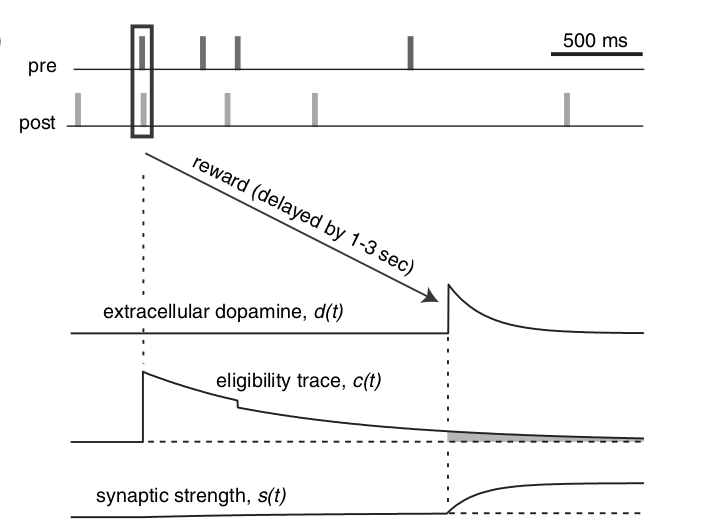
\includegraphics[width=\linewidth]{figures/izhikevich}
	\caption{Иллюстрация процесса усиления синаптической связи из работы \cite{izhikevich}. Происходит благодаря повышению уровня дофамина и имеюшейся у синапса «сигнальной отметки» (eligibility trace), которая возникла секундами раньше.}
	\label{fig:izhikevich}
\end{figure}


Cохранено предположение, что в синапсах, соединяющих два возбуждающих нейрона, действует спайковая пластичность, зависящая от времени. Модель Е. Ижикевича для дофамина была представлена в виде набора определяющих уравнений. Опираясь на них, для сети нейронов, где 80\% возбуждающие и 20\% ингибирующие, для норадреналина составлены следующие уравнения:


1) Динамика каждого нейрона такова, что потенциал мембраны $v$ каждого нейрона в каждый момент времени зависит от абстрактной переменной восстановления мембраны $u$ (новый потенциал в этой точке $\dot{v}$) \cite{tactile}:

\begin{equation} \label{eq:1}
\dot{v} = k (v - v_{rest})(v - v_{thresh}) - u + I
\end{equation}


\begin{equation} \label{eq:2}
%SD
% u =  a*b*(v - v_{rest}) - u 
\dot{u}=  a*b*(v - v_{rest}) - u
\end{equation}


\begin{equation}\label{eq:3}
if (v >= 30 [mV]) : \{v = - 65 [mV], u = u + 2 [mV]\}
\end{equation}


В нашей модели пороговый потенциал мембраны $v_{thresh}$ и потенциал покоя $v_{rest}$ являются константами, синаптический ток $I$ (внутри нейрона) имеет экспоненциальную форму. Спайк происходит, когда потенциал мембраны превышает $v_{thresh}$ (-50 mV), и после спайка потенциал мембраны восстанавливается: $v$ снижается до -65 mV, $u$ вырастает до 2 mV. Значение переменной $a$ установлено 0.02, переменная $b$ равна 0.2, коэффициент $k$ --- 1.


Синаптический вес $w$ (сила синаптической связи) изменяется в модели не напрямую \cite{stdp}, а модулируется через временную <<сигнальную отметку>> $c$, что показано в (\ref{eq:6}). Изменение <<сигнальной отметки>> $c$ в течение времени происходит по следующему закону (новое значение в конкретной точке --- $\dot{c}$):


\begin{equation}\label{eq:4}
\dot{c} =  -\frac{c}{\tau_c} + A^+e^{\frac{(t_{pre} - t_{post})}{\tau^+}}\delta(t - t_{post})  -A^-e^{  \frac{(t_{pre} - t_{post})}{\tau^-}}\delta(t - t_{pre} )
\end{equation}


где $t_{pre}$ и $t_{post}$ это время пресинаптического и постсинаптического спайков, $A^+$ и $A^-$ это амплитуды изменения синаптического веса, $\tau_+$ и $\tau_-$ --- константы затухания, $\delta(t)$ это дельта-функция Дирака, пошагово увеличивающая переменную $c$. Значение сигнальной отметки уменьшается с постоянной скоростью $\tau_c$. 


Концентрация норадреналина также влияет на модулирование синаптического веса \cite{nora1}\cite{nora2}, что показано в (\ref{eq:6}). Концентрация норадреналина $n$ уменьшается экспоненциально с течением времени (со скоростью $\tau_n$), а увеличивается в зависимости от неожиданных событий:


\begin{equation}\label{eq:5}
\dot{n} = -\frac{n}{\tau_n} + p_{nov}n (\delta(t - t_n)p_{rew} + \delta(t - t_n)p_{pun})
\end{equation}


где $p_{punish}$ это стрессовое событие (наказание), $p_{rew}$ это событие награды, $p_{nov}$ это вероятность того, что событие является новым и неожиданным. Концентрация норадреналина не может опуститься ниже нуля, и повышается из-за неожиданных событий как позитивной, так и негативной окраски.


Синаптический вес $w$ (сила синаптической связи) изменяется в модели пропорционально относительной концентрации норадреналина $n$ по сравнению с минимальной концентрацией ($b_n$), умноженной на значение сигнальной отметки $c$:

\begin{equation}\label{eq:6}
\dot{w} = c(n - b_n)
\end{equation}


Модель была протестирована на языке MATLAB, вместе с уже реализованными моделями серотонина и дофамина, в следующих условиях:
\begin{itemize}
\item Задана сеть из 1000 нейронов с синаптической пластичностью, зависящей от времени;
\item 100 синапсов на нейрон;
\item Максимальный вес синапса 5;
\item Потенциал покоя мембраны -65 mV;
\end{itemize}

\begin{figure}
	\centering
	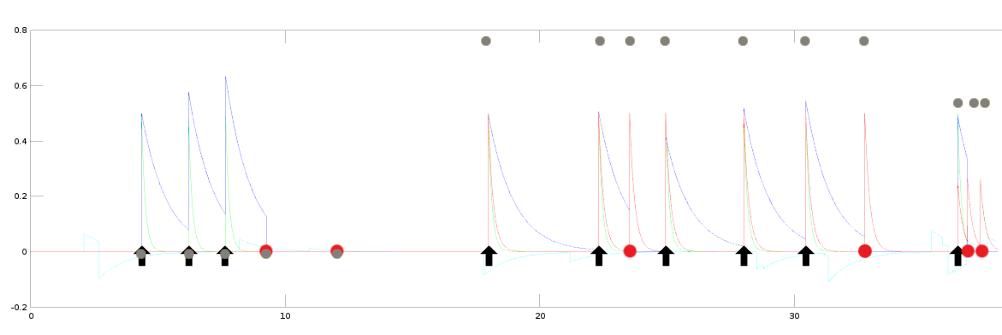
\includegraphics[width=\linewidth]{BIG_matlab_NA_with_NOV}
	\caption{Изменение концентрации норадреналина (красный), дофамина (зелёный) и серотонина (синий) в зависимости от примененных к ним стимулов: поощрение (чёрная стрелка), стресс (красный кружок), новизна (серый кружок).}
	\label{fig:matlab_NA}
\end{figure}

На рисунке ~\ref{fig:matlab_NA} изображён результат работы нейронной сети из 1000 нейронов в течение 500 миллисекунд, на которую подавались случайным образом события поощрения и стресса. Каждое из событий имело уровень неожиданности нулевой (полностью предсказуемое событие, первая треть временной шкалы), средний (последняя треть временной шкалы) или высокий (резкое, внезапное событие).
При абсолютной предсказуемости событий концентрация норадреналина не поднимается совсем, тогда как уровни серотонина и дофамина одинаково поднимаются от предсказуемой награды, от предсказуемого наказания (стресса) уровень серотонина обрушивается вниз, а дофамин на наказание не реагирует.
При событии резком, сколько-нибудь внезапном, будь то поощрение или наказание, концентрация норадреналина повышается; реакция серотонина и дофамина на эти события остаётся той же, что и когда они были «ожидаемы», «предсказаны» системой.


Полученные реакции соответствуют экспериментальным результатам исследовательских работ разных лет.\cite{viljoen, delaneytransmission, macaca} Поскольку результат, показанный моделью норадреналина в MATLAB, был убедителен, то модель была перенесена на язык c++ и добавлена в инструмент симуляции нейронных спайковых сетей NEST-2.12.0 в качестве нового модуля. Работа модуля была протестирована на простой модели из трёх нейронов: пресинаптический нейрон, постсинаптический нейрон и норадренергический нейрон. Модель симулировала процесс нейромодуляции, усиливающий связь между обычными нейронами в случае, если между ними произошёл спайк при высокой концентрации нейромодулятора норадреналин. Для этого к каждому из трёх нейронов были подключены генераторы спайков в 250 Гц и детекторы спайков. Модель была запущена дважды: с активацией норадреналина и без. Симуляции длились по 3000 миллисекунд.


\begin{figure}
	\centering
	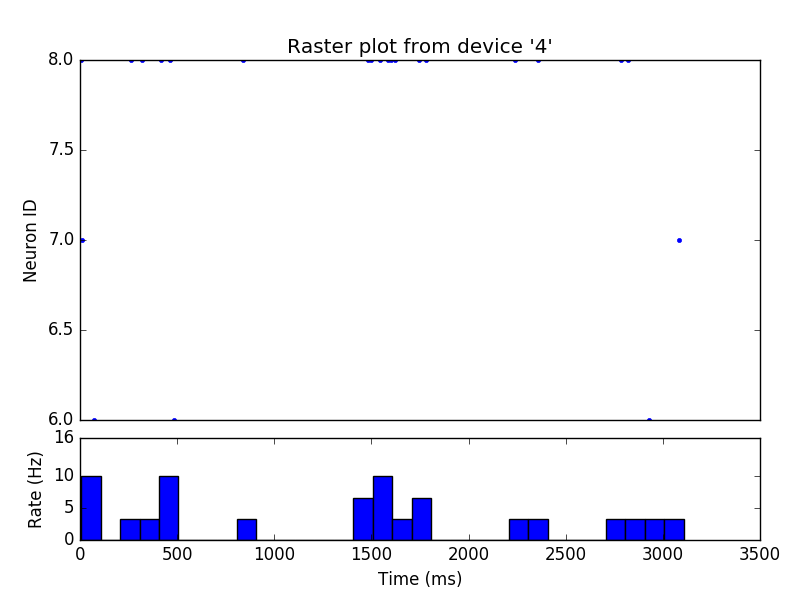
\includegraphics[width=\linewidth]{spikes_250}
	\caption{Спайковая активность на нейроне 6 (пресинаптический), нейроне 7 (постсинаптический), нейроне 8 (норадренергический). Группы спайков на 300 мс, 800 мс, 1500 мс, 2400 мс и 2700 мс разделены промежутками более 250 мс, что делает каждую из них неожиданными для алгоритма, определяющего неожиданность.}
	\label{fig:s_250}
\end{figure}

\begin{figure}
	\centering
	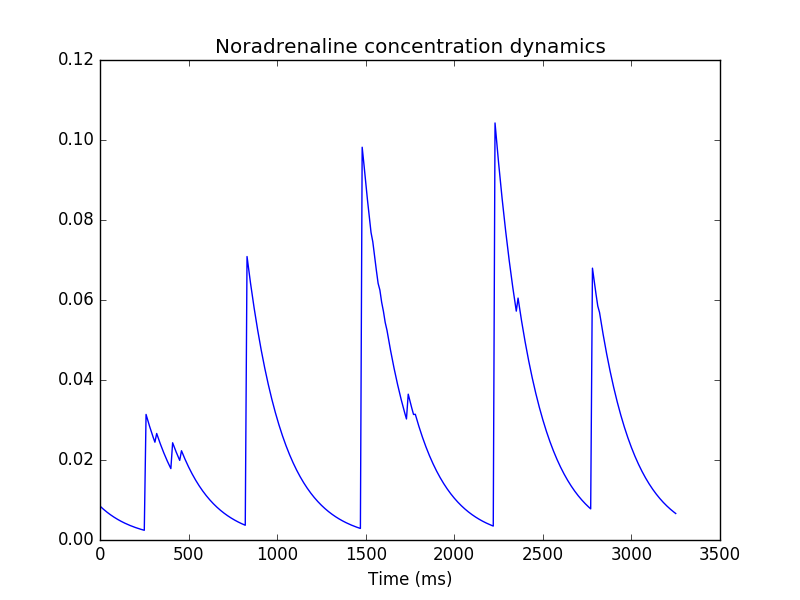
\includegraphics[width=\linewidth]{nora_dynamic_250}
	\caption{Динамика концентрации норадреналина.}
	\label{fig:nora_dynamic_250}
\end{figure}


На рисунке \ref{fig:s_250} показана спайковая активность каждого из трёх нейронов в эксперименте с активированным норадреналином. На рисунке \ref{fig:nora_dynamic_250} — изменение концентрации норадреналина со временем. Сильное увеличение концентрации наступает после относительно «длительного» отсутствия спайков, поскольку после «тишины» в 400 миллисекунд новый спайк имеет уже ненулевой фактор внезапности, считается неожиданным. В случае же спайков идущих подряд концентрация падает. То, как сочетание спайков и изменений концентрации повлияло на силу связи (вес синапса) между пресинаптическим и постсинаптическим нейронами, показывает рисунок \ref{fig:w_250}. Вес синапса растёт рывками, в соответствии с работой генераторов.

\begin{figure}
	\centering
	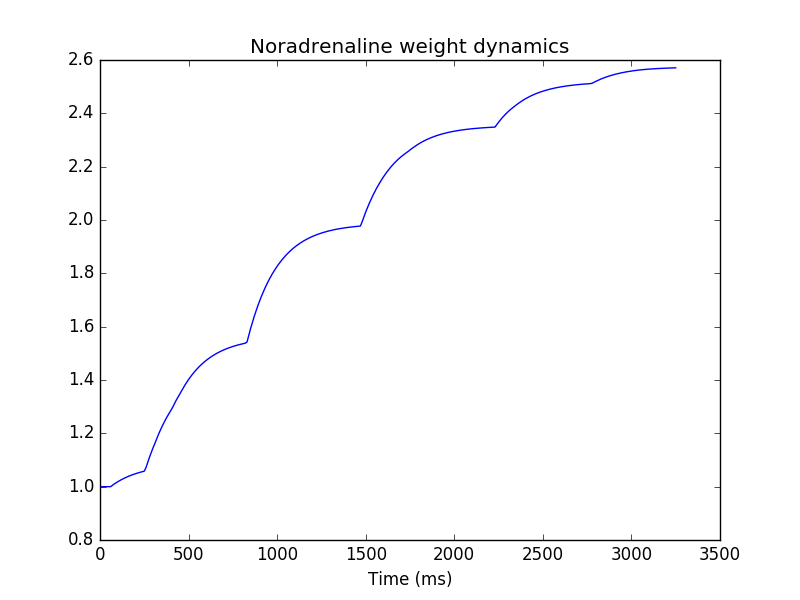
\includegraphics[width=\linewidth]{w_dynamic_250_with_nora}
	\caption{Изменение силы связи между пресинаптическим и постсинаптическим нейронами в присутствии норадреналина.}
	\label{fig:w_250}
\end{figure}

Второй, контрольный эксперимент без активации норадреналина показал, что без присутствия нейромодулятора сила связи между нейронами единична и не меняется на протяжении всей симуляции (рисунок \ref{fig:w_no_nora}).

\begin{figure}
	\centering
	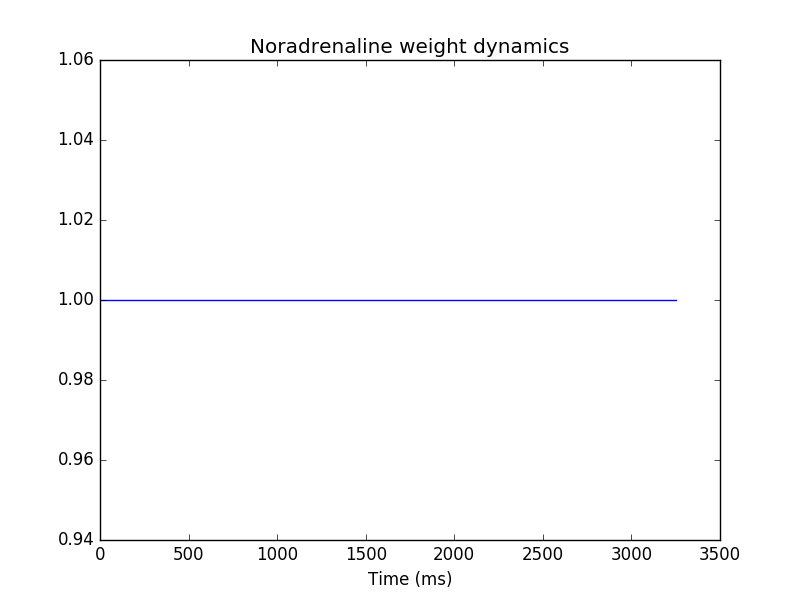
\includegraphics[width=\linewidth]{w_dynamic_250}
	\caption{Изменение силы связи между пресинаптическим и постсинаптическим нейронами в отсутствие нейромодуляторов.}
	\label{fig:w_no_nora}
\end{figure}